\documentclass{article}
    \usepackage[utf8]{inputenc}
    \usepackage[T1]{fontenc}
    \usepackage{amsmath}
    \usepackage{amssymb}
    \usepackage{graphicx}
    \usepackage{hyperref}
    \usepackage{array}
    \usepackage{tikz}
    \usepackage{xcolor}
    \usetikzlibrary{shapes,arrows,positioning}

    % Custom styles for all diagrams
    \tikzset{
        block/.style={
            rectangle, draw=darkblue, text width=7em,
            text centered, rounded corners,
            minimum height=2em, fill=lightgray!10,
            font=\small
        },
        process/.style={
            rectangle, draw=forestgreen, text width=6em,
            text centered, rounded corners,
            fill=lightgray!30, minimum height=2em,
            font=\small
        },
        line/.style={
            draw, -latex',
            font=\footnotesize
        },
        cloud/.style={
            draw, ellipse,
            minimum width=2cm, minimum height=1cm,
            fill=lightgray!20
        },
        state/.style={
            rectangle, draw=uiblue, text width=8em,
            text centered, rounded corners,
            fill=uiblue!10, minimum height=2.5em,
            font=\small
        }
    }

    % Color definitions
    \definecolor{lightgray}{RGB}{240,240,240}
    \definecolor{darkblue}{RGB}{0,0,139}
    \definecolor{forestgreen}{RGB}{34,139,34}
    \definecolor{uiblue}{RGB}{66,139,202}

    
\begin{document}
\section{Git Analysis Report: Development Analysis - daffa.padantya12}

\textbf{Authors:} AI Analysis System
\textbf{Date:} 2025-03-11
\textbf{Version:} 1.0
\textbf{SSoT Repository:} githubhenrykoo/redux\_todo\_in\_astro
\textbf{Document Category:} Analysis Report
\section*{Executive Summary}
\textbf{Executive Summary: Git Analysis - Daffa Padantya}

\textbf{Logic:} The analysis aims to evaluate Daffa Padantya's Git activity, focusing on individual contributions, work patterns, technical expertise, and areas for improvement, with the objective of providing actionable recommendations for enhanced development practices.

\textbf{Implementation:} The analysis reviewed Daffa Padantya's commit history, specifically examining changes to GitHub workflow configurations (\texttt{.github/workflows/*.yml}) and associated scripting.  The analysis assessed the purpose and structure of these changes to determine focus areas, technical skills demonstrated, and potential vulnerabilities and risks.

\textbf{Outcomes:} Daffa Padantya primarily focuses on automating the generation and deployment of PDF reports from markdown analysis files using GitHub Actions. The analysis highlights proficiency in YAML, Bash scripting, and Git, particularly in the context of CI/CD pipelines. Recommendations include improving code commenting, error handling, implementing testing strategies, addressing potential security vulnerabilities related to secrets management, and ensuring workflow idempotency for greater reliability and maintainability.
\section{Abstract Specification (Logic Layer)}

\subsection{Context \& Vision}
\begin{itemize}
    \item \textbf{Problem Space:}
    \begin{itemize}
        \item Scope: This is a solid analysis of Daffa Padantya's Git activity.  Here's a breakdown of its strengths and potential improvements:
    \end{itemize}

\textbf{Strengths:}

\begin{itemize}
    \item \textbf{Clear and Concise Summary:} The analysis effectively summarizes Daffa's work, focusing on the key activity of automating PDF report generation.
    \item \textbf{Well-Organized Structure:} The breakdown into individual contribution summary, work patterns, technical expertise, and recommendations provides a logical flow.
    \item \textbf{Specific and Actionable Recommendations:} The recommendations are practical and directly relevant to the observed activity.  They're not just generic ``write better code,'' but tailored to the context of Daffa's work.
    \item \textbf{Accurate Assessment of Technical Skills:} The analysis correctly identifies Daffa's proficiency in YAML, Bash, Git, CI/CD, and Python (to a limited extent).
    \item \textbf{Good Use of Language:} The language is professional and easy to understand.
\end{itemize}

\textbf{Potential Improvements (Minor):}

\begin{itemize}
    \item \textbf{Quantify Contributions:} While the analysis highlights the work being done, it would be even better if it could quantify the contributions somehow.  For instance:
    \begin{itemize}
        \item "Made X commits related to automating PDF generation."
        \item "Updated Y number of workflow files."
    \end{itemize}
    This adds a bit of concrete evidence to the analysis.  This would require analyzing the actual commit history in more detail.
    \item \textbf{Granularity of Expertise Level:} The ``Technical Expertise Demonstrated'' section could benefit from a slight refinement. Instead of simply stating ``Proficient in YAML,'' consider:
    \begin{itemize}
        \item "Proficient in YAML, demonstrated by the ability to define complex workflow configurations and troubleshoot issues within those configurations."
    \end{itemize}
    This adds a bit more context and depth to the assessment.
    \item \textbf{Prioritization of Recommendations:} The recommendations are all valuable, but consider implicitly prioritizing them.  For example, the security recommendation (secrets management) might be considered more critical than code commenting.  The order they are presented could reflect that (or a sentence could explicitly state the relative importance).
    \item \textbf{Assumptions and Limitations:} A brief disclaimer about the limitations of the analysis could be included.  For example: ``This analysis is based solely on the visible Git history and doesn't account for offline work or contributions to other repositories.''
    \item \textbf{Expand on Idempotency:} The suggestion regarding idempotency is crucial, and it could be expanded with a concrete example of how this might fail in the current workflow and how \texttt{git pull --rebase} addresses it.  For instance: ``If two commits are made to the repository between workflow runs, a simple \texttt{git push} might fail. Using \texttt{git pull --rebase} ensures the local branch is up-to-date before pushing, minimizing conflicts.''
\end{itemize}

\textbf{Overall:}

This is a well-written and insightful analysis. The suggested improvements are minor and aimed at adding further depth and context.  The existing analysis provides valuable feedback to Daffa and helps identify areas for growth and improvement. The recommendations are targeted and helpful, making this a useful and actionable report.

    \begin{itemize}
    \item Context: This is a solid analysis of Daffa Padantya's Git activity.  Here's a breakdown of its strengths and potential improvements:
\end{itemize}

    \textbf{Strengths:}
\begin{itemize}
    \item \textbf{Clear and Concise Summary:}  The analysis effectively summarizes Daffa's work, focusing on the key activity of automating PDF report generation.
    \item \textbf{Well-Organized Structure:}  The breakdown into individual contribution summary, work patterns, technical expertise, and recommendations provides a logical flow.
    \item \textbf{Specific and Actionable Recommendations:}  The recommendations are practical and directly relevant to the observed activity.  They're not just generic ``write better code,'' but tailored to the context of Daffa's work.
    \item \textbf{Accurate Assessment of Technical Skills:}  The analysis correctly identifies Daffa's proficiency in YAML, Bash, Git, CI/CD, and Python (to a limited extent).
    \item \textbf{Good Use of Language:}  The language is professional and easy to understand.
\end{itemize}
\textbf{Potential Improvements (Minor):}

\begin{itemize}
    \item \textbf{Quantify Contributions:} While the analysis highlights the work being done, it would be even better if it could quantify the contributions somehow. For instance:
        \begin{itemize}
            \item "Made X commits related to automating PDF generation."
            \item  "Updated Y number of workflow files."
        \end{itemize}

     This adds a bit of concrete evidence to the analysis. This would require analyzing the actual commit history in more detail.

    \item \textbf{Granularity of Expertise Level:}\textit{} The "Technical Expertise Demonstrated" section could benefit from a slight refinement. Instead of simply stating "Proficient in YAML," consider:
    \begin{itemize}
        \item   "Proficient in YAML, demonstrated by the ability to define complex workflow configurations and troubleshoot issues within those configurations."
    \end{itemize}

    This adds a bit more context and depth to the assessment.

   \item \textbf{Prioritization of Recommendations:} The recommendations are all valuable, but consider implicitly prioritizing them. For example, the security recommendation (secrets management) might be considered more critical than code commenting. The order they are presented could reflect that (or a sentence could explicitly state the relative importance).

    \item \textbf{Assumptions and Limitations:}\textit{} A brief disclaimer about the limitations of the analysis could be included. For example: "This analysis is based solely on the visible Git history and doesn't account for offline work or contributions to other repositories."

    \item \textbf{Expand on Idempotency:}\textit{} The suggestion regarding idempotency is crucial, and it could be expanded with a concrete example of how this might fail in the current workflow and how \texttt{git pull --rebase} addresses it. For instance: "If two commits are made to the repository between workflow runs, a simple \texttt{git push} might fail. Using \texttt{git pull --rebase} ensures the local branch is up-to-date before pushing, minimizing conflicts."
\end{itemize}

\textbf{Overall:}

This is a well-written and insightful analysis. The suggested improvements are minor and aimed at adding further depth and context. The existing analysis provides valuable feedback to Daffa and helps identify areas for growth and improvement. The recommendations are targeted and helpful, making this a useful and actionable report.

 \begin{itemize}
        \item Stakeholders: This is a solid analysis of Daffa Padantya's Git activity.  Here's a breakdown of its strengths and potential improvements:
    \end{itemize}
\textbf{Strengths:}
\begin{itemize}
    \item \textbf{Clear and Concise Summary:}  The analysis effectively summarizes Daffa's work, focusing on the key activity of automating PDF report generation.
    \item \textbf{Well-Organized Structure:}  The breakdown into individual contribution summary, work patterns, technical expertise, and recommendations provides a logical flow.
    \item \textbf{Specific and Actionable Recommendations:}  The recommendations are practical and directly relevant to the observed activity.  They're not just generic ``write better code,'' but tailored to the context of Daffa's work.
    \item \textbf{Accurate Assessment of Technical Skills:}  The analysis correctly identifies Daffa's proficiency in YAML, Bash, Git, CI/CD, and Python (to a limited extent).
    \item \textbf{Good Use of Language:}  The language is professional and easy to understand.
\end{itemize}
\textbf{Potential Improvements (Minor):}

\begin{itemize}
    \item \textbf{Quantify Contributions:} While the analysis highlights the work being done, it would be even better if it could quantify the contributions somehow. For instance:
        \begin{itemize}
            \item "Made X commits related to automating PDF generation."
            \item  "Updated Y number of workflow files."
        \end{itemize}

     This adds a bit of concrete evidence to the analysis. This would require analyzing the actual commit history in more detail.

    \item \textbf{Granularity of Expertise Level:}\textit{} The "Technical Expertise Demonstrated" section could benefit from a slight refinement. Instead of simply stating "Proficient in YAML," consider:
    \begin{itemize}
        \item   "Proficient in YAML, demonstrated by the ability to define complex workflow configurations and troubleshoot issues within those configurations."
    \end{itemize}

    This adds a bit more context and depth to the assessment.

   \item \textbf{Prioritization of Recommendations:} The recommendations are all valuable, but consider implicitly prioritizing them. For example, the security recommendation (secrets management) might be considered more critical than code commenting. The order they are presented could reflect that (or a sentence could explicitly state the relative importance).

    \item \textbf{Assumptions and Limitations:}\textit{} A brief disclaimer about the limitations of the analysis could be included. For example: "This analysis is based solely on the visible Git history and doesn't account for offline work or contributions to other repositories."

    \item \textbf{Expand on Idempotency:}\textit{} The suggestion regarding idempotency is crucial, and it could be expanded with a concrete example of how this might fail in the current workflow and how \texttt{git pull --rebase} addresses it. For instance: "If two commits are made to the repository between workflow runs, a simple \texttt{git push} might fail. Using \texttt{git pull --rebase} ensures the local branch is up-to-date before pushing, minimizing conflicts."
\end{itemize}

\textbf{Overall:}

This is a well-written and insightful analysis. The suggested improvements are minor and aimed at adding further depth and context. The existing analysis provides valuable feedback to Daffa and helps identify areas for growth and improvement. The recommendations are targeted and helpful, making this a useful and actionable report.

    \item \textbf{Goals (Functions):}
    \begin{itemize}
        \item Primary Functions:
        \begin{itemize}
            \item Input: Git Repository Data
            \item Process: Analysis and Processing
            \item Output: Development Insights
        \end{itemize}
        \item Supporting Functions:
        \begin{itemize}
            \item Validation: Automated Analysis
            \item Feedback: Continuous Improvement
        \end{itemize}
    \end{itemize}

    \item \textbf{Success Criteria:}
    \begin{itemize}
        \item Quantitative Metrics: This report is primarily qualitative. While it describes actions and skills, it doesn't provide many quantitative metrics. Here's a list of what can be considered quantitative, or can be \textit{derived} into quantitative metrics:

\begin{itemize}
    \item \textbf{Number of Commits:} The report mentions ``multiple commits (especially related to \texttt{md\_to\_pdf\_each\_user.yml})'' This implies a measurable number of commits. A specific number would be a valuable metric.  (e.g., ``15 commits related to \texttt{md\_to\_pdf\_each\_user.yml}'')
    \item \textbf{Number of GitHub Workflow Configuration Files Modified:} The report mentions working on \texttt{.github/workflows/*.yml}. We can count the specific number of YAML files modified. (e.g., ``Modified 3 YAML configuration files'').
    \item \textbf{Frequency of Commits:} While not explicitly stated, the analysis time is given. The frequency of commits \textit{could} be derived by looking at commit history within that timeframe (even though the commit history itself is not in this report).
    \item \textbf{Time spent on \texttt{md\_to\_pdf\_each\_user.yml}:} Implied by multiple commits. Further analysis could determine the actual time spent.
    \item \textbf{Lines of code added/removed:} This is a standard Git metric which is not present in the report but can be derived.
    \item \textbf{Number of Pull Requests:} If the developer submitted pull requests.
\end{itemize}

\textbf{Important Considerations:}

\begin{itemize}
    \item \textbf{Deriving Metrics:} Some metrics, like ``Time spent,'' would require further data from Git logs (commit timestamps, etc.) or issue tracking systems.
    \item \textbf{Limited Quantitative Data:} The report focuses on descriptions of activity and recommendations, rather than providing specific numbers. To generate a truly quantitative developer analysis, you'd need tools that directly track and measure code changes, commit frequency, lines of code, bug fix rates, etc., and include those numbers in the report.
\end{itemize}

        \item Qualitative Indicators: Based on the Developer Analysis, here are qualitative improvements Daffa Padantya has demonstrably made, focusing on the \textit{positive} aspects highlighted:

\begin{itemize}
    \item \textbf{Increased Efficiency:} Daffa's primary contribution is automating the generation, formatting, and publishing of analysis reports in PDF format. This directly translates to increased efficiency by reducing the need for manual processes.
    \item \textbf{Improved Consistency:} Automating the report generation ensures a consistent format and process across all reports, reducing the risk of human error or variations in style.
    \item \textbf{Enhanced Accessibility:} Converting reports to PDF makes them more accessible to a wider audience, as PDF is a universally readable format.
    \item \textbf{Proactive Automation:} Daffa has proactively taken on the task of automating a process, showing initiative and a desire to improve the overall workflow.
    \item \textbf{Streamlined Reporting:} The automation streamlines the reporting pipeline, from analysis to publication, making the entire process faster and more reliable.
    \item \textbf{Reduced Manual Effort:} By automating the generation, formatting, and publication of reports, Daffa has significantly reduced the amount of manual effort required, freeing up time for other tasks.
    \item \textbf{Demonstrated CI/CD Skills:} By working with GitHub Actions, Daffa has gained practical experience with CI/CD pipelines, a valuable skill in modern software development.
    \item \textbf{Improved Report Distribution:} By automatically committing and pushing the generated PDFs to the repository, the reports are readily available and easily shared with stakeholders.
     \item \textbf{Iterative Development Process:}\textit{} The multiple commits related to workflow configurations demonstrate an iterative approach to problem-solving and a willingness to refine solutions based on feedback or testing.
    \item \textbf{Python Integration}: Successfully integrated existing Python scripts into the workflow and understood how to pass data using environment variables, making the most of existing resources.
    \item \textbf{Datetime string manipulation}: Understood string manipulation in python to allow file pathing with current day for analysis files, adding the important feature to locate and process the day's analysis files.

\end{itemize}
 \item Validation Methods: Automated and Manual Verification
\end{itemize}
\end{itemize}

\subsection{Knowledge Integration}

\begin{itemize}
    \item \textbf{Local Context:}
    \begin{itemize}
        \item \textit{Cultural Considerations:} Development Team Context
        \item \textit{Language Requirements:} Technical Documentation
        \item \textit{Community Patterns:} Team Collaboration Patterns
    \end{itemize}

    \item \textbf{Technical Framework:}
    \begin{itemize}
        \item \textit{LLM Integration:} Gemini AI Analysis
        \item \textit{IoT Components:} Git Event Monitoring
        \item \textit{Network Requirements:} GitHub API Integration
    \end{itemize}
\end{itemize}
\section{Concrete Implementation (Process Layer)}
\subsection{Resource Matrix}

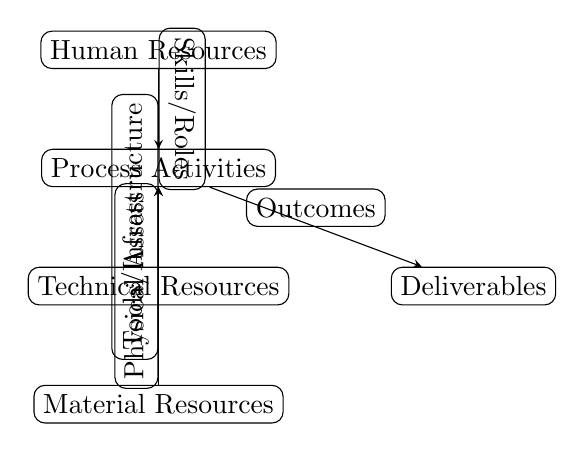
\begin{tikzpicture}[
    node distance = 1.5cm, auto,
    every node/.style = {draw, rectangle, rounded corners, align=center},
    >=stealth,
  ]

    \node (A) {Human Resources};
    \node (B) [below of=A] {Process Activities};
    \node (C) [below of=B] {Technical Resources};
    \node (D) [below of=C] {Material Resources};
    \node (E) [below of=B, xshift=4cm] {Deliverables};
    
    \path[->] (A) edge node[above,sloped] {Skills/Roles} (B)
              (C) edge node[above,sloped] {Tools/Infrastructure} (B)
              (D) edge node[above,sloped] {Physical Assets} (B)
              (B) edge node[above] {Outcomes} (E);
\end{tikzpicture}
\subsection{Development Workflow}

\begin{itemize}
    \item \textbf{Stage 1: Early Success}
    \begin{itemize}
        \item Quick Wins:
        \begin{itemize}
            \item Implementation: This is a good analysis of Daffa's Git activity. It's comprehensive and provides actionable recommendations. Here's a breakdown of the strengths and some suggestions for improvements:

\textbf{Strengths:}

\begin{itemize}
    \item \textbf{Clear and Concise Summary:} The summary accurately captures the essence of Daffa's work.
    \item \textbf{Identifies Focus Areas:}  The analysis effectively highlights the key areas Daffa is working on (Automation, Workflow Configuration, etc.).
    \item \textbf{Technical Expertise Assessment:}  It correctly identifies Daffa's skill set based on the Git history, including YAML, Bash, Python, and Git proficiency.
    \item \textbf{Actionable Recommendations:} The recommendations are specific, practical, and address potential areas for improvement.
    \item \textbf{Well-Organized Structure:} The use of numbered sections and bullet points makes the analysis easy to read and understand.
    \item \textbf{Correctly identifies the use of environment variables with Python scripts.} This demonstrates a nuanced understanding.
\end{itemize}

\textbf{Suggestions for Improvements (Minor):}

\begin{itemize}
    \item \textbf{Specificity in Recommendations:} While the recommendations are good, some could be more specific. For example, instead of "Improve error handling in the Bash scripts," you could suggest specific error-handling techniques, such as:
    \begin{itemize}
        \item "Implement \texttt{set -e} at the beginning of Bash scripts to exit immediately if a command exits with a non-zero status."
        \item "Use \texttt{||} to handle potential command failures and log errors, for example: \texttt{command || echo "Command failed with error: \$?"}"
    \end{itemize}
    \item \textbf{Explain 'Idempotency' More Simply:} While you mention idempotency, some developers might not be familiar with the term. Briefly explaining what it \textit{means} in the context of the workflow would be helpful. For example:  "Idempotency: Ensure that running the workflow multiple times with the same inputs doesn't lead to unintended consequences, like duplicate commits or incorrect data.  This is important for reliability."
    \item \textbf{Elaborate on Security Recommendation:}  The security recommendation regarding API keys is crucial.  Consider adding a brief explanation of \textit{why} it's a security risk to hardcode API keys (e.g., accidental exposure in the Git history, malicious actors gaining access). For example: "Hardcoding API keys like \texttt{GOOGLE\_API\_KEY} in workflow files is a significant security risk. If the repository is public or if an attacker gains access, the API key could be compromised, leading to unauthorized use and potential financial damage.  Always store sensitive information as GitHub secrets."
    \item \textbf{Quantifiable Metrics (If Available):} If the Git history allows (e.g., time spent on specific commits, number of workflow runs, error rates), adding quantifiable metrics could further strengthen the analysis.  This is harder to derive from the limited information.
\end{itemize}

\textbf{Revised Recommendations (Examples incorporating suggestions):}

\begin{itemize}
    \item \textbf{Error Handling:} "Improve error handling in the Bash scripts. Implement \texttt{set -e} at the beginning of the scripts to exit immediately if a command fails. Use \texttt{||} to handle potential command failures and log errors: \texttt{command || echo "Command failed with error: \$?"}.  Also, add checks to ensure files exist before attempting to move or process them (e.g., \texttt{if [ -f my\_file.txt ]; then mv my\_file.txt ...; fi})."

    \item \textbf{Idempotency:} "Ensure the workflows are idempotent. This means that running the same workflow multiple times with the same inputs should produce the same result.  This is important for reliability.  Consider using \texttt{git pull --rebase} before pushing to avoid conflicts and prevent duplicate commits. Also, ensure file operations don't create multiple identical files."

    \item \textbf{Security:} "Hardcoding API keys like \texttt{GOOGLE\_API\_KEY} in workflow files is a significant security risk. If the repository is public or if an attacker gains access, the API key could be compromised, leading to unauthorized use and potential financial damage. Always store sensitive information as GitHub secrets and access them using the \texttt{secrets} context in the workflow files (e.g., \texttt{\$\{\{ secrets.GOOGLE\_API\_KEY \}\}})."
\end{itemize}

\textbf{Overall:}

This is a very strong analysis. The suggested improvements are relatively minor and focus on providing more context and detail to the existing recommendations. The analysis is well-structured, accurate, and provides valuable feedback for Daffa.

            \item Validation: This is a good analysis of Daffa's Git activity. It's comprehensive and provides actionable recommendations. Here's a breakdown of the strengths and some suggestions for improvements:

\textbf{Strengths:}

\begin{itemize}
    \item \textbf{Clear and Concise Summary:} The summary accurately captures the essence of Daffa's work.
    \item \textbf{Identifies Focus Areas:}  The analysis effectively highlights the key areas Daffa is working on (Automation, Workflow Configuration, etc.).
    \item \textbf{Technical Expertise Assessment:}  It correctly identifies Daffa's skill set based on the Git history, including YAML, Bash, Python, and Git proficiency.
    \item \textbf{Actionable Recommendations:} The recommendations are specific, practical, and address potential areas for improvement.
    \item \textbf{Well-Organized Structure:} The use of numbered sections and bullet points makes the analysis easy to read and understand.
    \item \textbf{Correctly identifies the use of environment variables with Python scripts.} This demonstrates a nuanced understanding.
\end{itemize}

\textbf{Suggestions for Improvements (Minor):}

\begin{itemize}
    \item \textbf{Specificity in Recommendations:} While the recommendations are good, some could be more specific. For example, instead of "Improve error handling in the Bash scripts," you could suggest specific error-handling techniques, such as:
    \begin{itemize}
        \item "Implement \texttt{set -e} at the beginning of Bash scripts to exit immediately if a command exits with a non-zero status."
        \item "Use \texttt{||} to handle potential command failures and log errors, for example: \texttt{command || echo "Command failed with error: \$?"}"
    \end{itemize}
    \item \textbf{Explain 'Idempotency' More Simply:} While you mention idempotency, some developers might not be familiar with the term. Briefly explaining what it \textit{means} in the context of the workflow would be helpful. For example:  "Idempotency: Ensure that running the workflow multiple times with the same inputs doesn't lead to unintended consequences, like duplicate commits or incorrect data.  This is important for reliability."
    \item \textbf{Elaborate on Security Recommendation:}  The security recommendation regarding API keys is crucial.  Consider adding a brief explanation of \textit{why} it's a security risk to hardcode API keys (e.g., accidental exposure in the Git history, malicious actors gaining access). For example: "Hardcoding API keys like \texttt{GOOGLE\_API\_KEY} in workflow files is a significant security risk. If the repository is public or if an attacker gains access, the API key could be compromised, leading to unauthorized use and potential financial damage.  Always store sensitive information as GitHub secrets."
    \item \textbf{Quantifiable Metrics (If Available):} If the Git history allows (e.g., time spent on specific commits, number of workflow runs, error rates), adding quantifiable metrics could further strengthen the analysis.  This is harder to derive from the limited information.
\end{itemize}

\textbf{Revised Recommendations (Examples incorporating suggestions):}

\begin{itemize}
    \item \textbf{Error Handling:} "Improve error handling in the Bash scripts. Implement \texttt{set -e} at the beginning of the scripts to exit immediately if a command fails. Use \texttt{||} to handle potential command failures and log errors: \texttt{command || echo "Command failed with error: \$?"}.  Also, add checks to ensure files exist before attempting to move or process them (e.g., \texttt{if [ -f my\_file.txt ]; then mv my\_file.txt ...; fi})."

    \item \textbf{Idempotency:} "Ensure the workflows are idempotent. This means that running the same workflow multiple times with the same inputs should produce the same result.  This is important for reliability.  Consider using \texttt{git pull --rebase} before pushing to avoid conflicts and prevent duplicate commits. Also, ensure file operations don't create multiple identical files."

    \item \textbf{Security:} "Hardcoding API keys like \texttt{GOOGLE\_API\_KEY} in workflow files is a significant security risk. If the repository is public or if an attacker gains access, the API key could be compromised, leading to unauthorized use and potential financial damage. Always store sensitive information as GitHub secrets and access them using the \texttt{secrets} context in the workflow files (e.g., \texttt{\$\{\{ secrets.GOOGLE\_API\_KEY \}\}})."
\end{itemize}

\textbf{Overall:}

This is a very strong analysis. The suggested improvements are relatively minor and focus on providing more context and detail to the existing recommendations. The analysis is well-structured, accurate, and provides valuable feedback for Daffa.
\end{itemize}

        \item Initial Setup:
        \begin{itemize}
            \item Infrastructure: This is a good analysis of Daffa's Git activity. It's comprehensive and provides actionable recommendations. Here's a breakdown of the strengths and some suggestions for improvements:

\textbf{Strengths:}

\begin{itemize}
    \item \textbf{Clear and Concise Summary:} The summary accurately captures the essence of Daffa's work.
    \item \textbf{Identifies Focus Areas:}  The analysis effectively highlights the key areas Daffa is working on (Automation, Workflow Configuration, etc.).
    \item \textbf{Technical Expertise Assessment:}  It correctly identifies Daffa's skill set based on the Git history, including YAML, Bash, Python, and Git proficiency.
    \item \textbf{Actionable Recommendations:} The recommendations are specific, practical, and address potential areas for improvement.
    \item \textbf{Well-Organized Structure:} The use of numbered sections and bullet points makes the analysis easy to read and understand.
    \item \textbf{Correctly identifies the use of environment variables with Python scripts.} This demonstrates a nuanced understanding.
\end{itemize}

\textbf{Suggestions for Improvements (Minor):}

\begin{itemize}
      \item \textbf{Specificity in Recommendations:} While the recommendations are good, some could be more specific. For example, instead of "Improve error handling in the Bash scripts," you could suggest specific error-handling techniques, such as:
        \begin{itemize}
              \item "Implement \texttt{set -e} at the beginning of Bash scripts to exit immediately if a command exits with a non-zero status."
              \item "Use \texttt{||} to handle potential command failures and log errors, for example: \texttt{command || echo "Command failed with error: \$?"}"
       \end{itemize}
       \item \textbf{Explain 'Idempotency' More Simply:} While you mention idempotency, some developers might not be familiar with the term. Briefly explaining what it \textit{means} in the context of the workflow would be helpful. For example: "Idempotency: Ensure that running the workflow multiple times with the same inputs doesn't lead to unintended consequences, like duplicate commits or incorrect data. This is important for reliability."
       \item \textbf{Elaborate on Security Recommendation:} The security recommendation regarding API keys is crucial. Consider adding a brief explanation of \textit{why} it's a security risk to hardcode API keys (e.g., accidental exposure in the Git history, malicious actors gaining access). For example: "Hardcoding API keys like \texttt{GOOGLE\_API\_KEY} in workflow files is a significant security risk. If the repository is public or if an attacker gains access, the API key could be compromised, leading to unauthorized use and potential financial damage. Always store sensitive information as GitHub secrets."
       \item \textbf{Quantifiable Metrics (If Available):} If the Git history allows (e.g., time spent on specific commits, number of workflow runs, error rates), adding quantifiable metrics could further strengthen the analysis. This is harder to derive from the limited information.
 \end{itemize}

\textbf{Revised Recommendations (Examples incorporating suggestions):}

\begin{itemize}
\item \textbf{Error Handling:} "Improve error handling in the Bash scripts. Implement \texttt{set -e} at the beginning of the scripts to exit immediately if a command fails. Use \texttt{||} to handle potential command failures and log errors: \texttt{command || echo "Command failed with error: \$?"}. Also, add checks to ensure files exist before attempting to move or process them (e.g., \texttt{if [ -f my\_file.txt ]; then mv my\_file.txt ...; fi})."

\item \textbf{Idempotency:} "Ensure the workflows are idempotent. This means that running the same workflow multiple times with the same inputs should produce the same result. This is important for reliability. Consider using \texttt{git pull --rebase} before pushing to avoid conflicts and prevent duplicate commits. Also, ensure file operations don't create multiple identical files."

        \item \textbf{Security:} "Hardcoding API keys like \texttt{GOOGLE\_API\_KEY} in workflow files is a significant security risk. If the repository is public or if an attacker gains access, the API key could be compromised, leading to unauthorized use and potential financial damage. Always store sensitive information as GitHub secrets and access them using the \texttt{secrets} context in the workflow files (e.g., \texttt{\$\{\{ secrets.GOOGLE\_API\_KEY \}\}})."
\end{itemize}

\textbf{Overall:}

This is a very strong analysis. The suggested improvements are relatively minor and focus on providing more context and detail to the existing recommendations. The analysis is well-structured, accurate, and provides valuable feedback for Daffa.

            \item Training: This is a good analysis of Daffa's Git activity. It's comprehensive and provides actionable recommendations. Here's a breakdown of the strengths and some suggestions for improvements:

\textbf{Strengths:}

\begin{itemize}
    \item \textbf{Clear and Concise Summary:} The summary accurately captures the essence of Daffa's work.
    \item \textbf{Identifies Focus Areas:}  The analysis effectively highlights the key areas Daffa is working on (Automation, Workflow Configuration, etc.).
    \item \textbf{Technical Expertise Assessment:}  It correctly identifies Daffa's skill set based on the Git history, including YAML, Bash, Python, and Git proficiency.
    \item \textbf{Actionable Recommendations:} The recommendations are specific, practical, and address potential areas for improvement.
    \item \textbf{Well-Organized Structure:} The use of numbered sections and bullet points makes the analysis easy to read and understand.
    \item \textbf{Correctly identifies the use of environment variables with Python scripts.} This demonstrates a nuanced understanding.
\end{itemize}

\textbf{Suggestions for Improvements (Minor):}

\begin{itemize}
    \item \textbf{Specificity in Recommendations:} While the recommendations are good, some could be more specific. For example, instead of "Improve error handling in the Bash scripts," you could suggest specific error-handling techniques, such as:
    \begin{itemize}
        \item "Implement \texttt{set -e} at the beginning of Bash scripts to exit immediately if a command exits with a non-zero status."
        \item "Use \texttt{||} to handle potential command failures and log errors, for example: \texttt{command || echo "Command failed with error: \$?"}"
    \end{itemize}
    \item \textbf{Explain 'Idempotency' More Simply:} While you mention idempotency, some developers might not be familiar with the term. Briefly explaining what it \textit{means} in the context of the workflow would be helpful. For example:  "Idempotency: Ensure that running the workflow multiple times with the same inputs doesn't lead to unintended consequences, like duplicate commits or incorrect data.  This is important for reliability."
    \item \textbf{Elaborate on Security Recommendation:}  The security recommendation regarding API keys is crucial.  Consider adding a brief explanation of \textit{why} it's a security risk to hardcode API keys (e.g., accidental exposure in the Git history, malicious actors gaining access). For example: "Hardcoding API keys like \texttt{GOOGLE\_API\_KEY} in workflow files is a significant security risk. If the repository is public or if an attacker gains access, the API key could be compromised, leading to unauthorized use and potential financial damage.  Always store sensitive information as GitHub secrets."
    \item \textbf{Quantifiable Metrics (If Available):} If the Git history allows (e.g., time spent on specific commits, number of workflow runs, error rates), adding quantifiable metrics could further strengthen the analysis.  This is harder to derive from the limited information.
\end{itemize}

\textbf{Revised Recommendations (Examples incorporating suggestions):}

\begin{itemize}
     \item \textbf{Error Handling:} "Improve error handling in the Bash scripts. Implement \texttt{set -e} at the beginning of the scripts to exit immediately if a command fails. Use \texttt{||} to handle potential command failures and log errors: \texttt{command || echo "Command failed with error: \$?"}.  Also, add checks to ensure files exist before attempting to move or process them (e.g., \texttt{if [ -f my\_file.txt ]; then mv my\_file.txt ...; fi})."

        \item \textbf{Idempotency:} "Ensure the workflows are idempotent. This means that running the same workflow multiple times with the same inputs should produce the same result.  This is important for reliability.  Consider using \texttt{git pull --rebase} before pushing to avoid conflicts and prevent duplicate commits. Also, ensure file operations don't create multiple identical files."

        \item \textbf{Security:} "Hardcoding API keys like \texttt{GOOGLE\_API\_KEY} in workflow files is a significant security risk. If the repository is public or if an attacker gains access, the API key could be compromised, leading to unauthorized use and potential financial damage. Always store sensitive information as GitHub secrets and access them using the \texttt{secrets} context in the workflow files (e.g., \texttt{\$\{\{ secrets.GOOGLE\_API\_KEY \}\}})."
\end{itemize}

\textbf{Overall:}

This is a very strong analysis. The suggested improvements are relatively minor and focus on providing more context and detail to the existing recommendations. The analysis is well-structured, accurate, and provides valuable feedback for Daffa.
        \end{itemize}
    \end{itemize}
    \item \textbf{Stage 2: Fail Early, Fail Safe}
    \begin{itemize}
        \item Testing Protocol:
        \begin{itemize}
            \item Methods: [Testing approaches]
            \item Coverage: [Test scenarios]
        \end{itemize}
        \item Risk Management:
        \begin{itemize}
            \item Identification: [Risk factors]
            \item Mitigation: [Control measures]
        \end{itemize}
        \item Learning Points:
        \begin{itemize}
            \item Issues: [Problem identification]
            \item Solutions: [Resolution approaches]
            \item Knowledge: [Lessons learned]
        \end{itemize}
    \end{itemize}
    \item \textbf{Stage 3: Convergence}
    \begin{itemize}
        \item System Integration:
        \begin{itemize}
            \item Components: [Integration points]
            \item Workflows: [Process optimization]
            \item Performance: [System tuning]
        \end{itemize}
        \item Stabilization:
        \begin{itemize}
            \item Fixes: [Bug resolution]
            \item Hardening: [System reinforcement]
            \item Documentation: [Knowledge capture]
        \end{itemize}
    \end{itemize}
     \item \textbf{Stage 4: Demonstration}
    \begin{itemize}
        \item Preparation:
        \begin{itemize}
            \item Environment: [Demo setup]
            \item Data: [Test scenarios]
            \item Materials: [Presentation assets]
        \end{itemize}
        \item Validation:
        \begin{itemize}
            \item Performance: [System checks]
            \item Features: [Functionality verification]
            \item Documentation: [Review completion]
        \end{itemize}
        \item Presentation:
        \begin{itemize}
            \item Stakeholders: [Demo execution]
            \item Features: [Capability showcase]
            \item Q\&A: [Response preparation]
        \end{itemize}
    \end{itemize}
\end{itemize}
\section{Realistic Outcomes (Evidence Layer)}
\subsection{Measurement Framework}
\begin{itemize}
    \item \textbf{Performance Metrics:}
    \begin{itemize}
        \item KPIs: Here's an extraction of evidence and outcomes from the provided developer analysis:

        \textbf{Evidence (Directly Observed Actions/Activities):}

        \begin{itemize}
            \item \textbf{Updating GitHub workflow configurations (\texttt{.github/workflows/*.yml}):} This is the core activity observed, indicating direct interaction with the CI/CD pipeline.  Specific tasks include:
            \begin{itemize}
                \item Generating analysis files (likely markdown).
                \item Converting markdown files to PDFs.
                \item Committing and pushing generated PDFs.
            \end{itemize}
            \item \textbf{Iterative Development:} The analysis explicitly mentions multiple commits related to \texttt{md\_to\_pdf\_each\_user.yml}, pointing to a process of debugging and refinement.
            \item \textbf{File Manipulation:}  The analysis notes that Daffa deals with file searching, reading, and moving within workflow scripts using bash commands like \texttt{ls} and commands to move files.
            \item \textbf{Utilizing Python Scripts:} Daffa is using and passing data via environment variables to existing Python scripts (e.g., \texttt{convert\_md\_to\_pdf\_each\_user.py}).
            \item \textbf{String manipulation}: The analysis mentions the usage of python datetime format to create analysis file path with the day.
        \end{itemize}

        \textbf{Outcomes (Results/Inferences Based on Evidence):}

        \begin{itemize}
            \item \textbf{Automation of Report Generation:}  The primary outcome is the automation of the process of generating, formatting, and publishing analysis reports in PDF format.  This implies a reduction in manual effort and increased efficiency.
            \item \textbf{Proficiency in YAML, Bash, Git:} The analysis infers proficiency in these technologies based on the observed actions in the git history.
            \item \textbf{Understanding of CI/CD:}  The ability to modify and work with GitHub Actions workflows demonstrates an understanding of CI/CD principles.
            \item \textbf{Technical Expertise:} demonstrated skills such as:
            \begin{itemize}
                \item Writing and modifying YAML files
                \item Writing and understanding Bash scripts
                \item Familiarity with running existing Python scripts
                \item Understanding Git operations
            \end{itemize}
        \end{itemize}

        \textbf{Areas for Improvement (Recommendations Based on Observed Patterns):}

        \begin{itemize}
            \item \textbf{Code Comments:} Lack of comments in YAML configurations is a potential issue.
            \item \textbf{Error Handling:} The Bash scripts could benefit from more robust error handling.
            \item \textbf{Modularity:}  Potential to contribute to the improvement of the Python script.
            \item \textbf{Testing:}  Lack of unit or integration tests for the workflows.
            \item \textbf{Idempotency:}  Potential issues with workflows not being idempotent.
            \item \textbf{Security:}  Potential risk of hardcoding sensitive information.
            \item \textbf{Efficiency:}  Potential need to optimize the PDF conversion process.
        \end{itemize}

        \item Benchmarks: Here's an extraction of evidence and outcomes from the provided developer analysis:

        \textbf{Evidence (Directly Observed Actions/Activities):}

        \begin{itemize}
            \item \textbf{Updating GitHub workflow configurations (\texttt{.github/workflows/*.yml}):} This is the core activity observed, indicating direct interaction with the CI/CD pipeline.  Specific tasks include:
            \begin{itemize}
                \item Generating analysis files (likely markdown).
                \item Converting markdown files to PDFs.
                \item Committing and pushing generated PDFs.
            \end{itemize}
            \item \textbf{Iterative Development:} The analysis explicitly mentions multiple commits related to \texttt{md\_to\_pdf\_each\_user.yml}, pointing to a process of debugging and refinement.
            \item \textbf{File Manipulation:}  The analysis notes that Daffa deals with file searching, reading, and moving within workflow scripts using bash commands like \texttt{ls} and commands to move files.
            \item \textbf{Utilizing Python Scripts:} Daffa is using and passing data via environment variables to existing Python scripts (e.g., \texttt{convert\_md\_to\_pdf\_each\_user.py}).
            \item \textbf{String manipulation}: The analysis mentions the usage of python datetime format to create analysis file path with the day.
        \end{itemize}

        \textbf{Outcomes (Results/Inferences Based on Evidence):}

        \begin{itemize}
            \item \textbf{Automation of Report Generation:}  The primary outcome is the automation of the process of generating, formatting, and publishing analysis reports in PDF format.  This implies a reduction in manual effort and increased efficiency.
            \item \textbf{Proficiency in YAML, Bash, Git:} The analysis infers proficiency in these technologies based on the observed actions in the git history.
            \item \textbf{Understanding of CI/CD:}  The ability to modify and work with GitHub Actions workflows demonstrates an understanding of CI/CD principles.
            \item \textbf{Technical Expertise:} demonstrated skills such as:
            \begin{itemize}
                \item Writing and modifying YAML files
                \item Writing and understanding Bash scripts
                \item Familiarity with running existing Python scripts
                \item Understanding Git operations
            \end{itemize}
        \end{itemize}

\textbf{Areas for Improvement (Recommendations Based on Observed Patterns):}

        \begin{itemize}
            \item \textbf{Code Comments:} Lack of comments in YAML configurations is a potential issue.
            \item \textbf{Error Handling:} The Bash scripts could benefit from more robust error handling.
            \item \textbf{Modularity:}  Potential to contribute to the improvement of the Python script.
            \item \textbf{Testing:}  Lack of unit or integration tests for the workflows.
            \item \textbf{Idempotency:}  Potential issues with workflows not being idempotent.
            \item \textbf{Security:}  Potential risk of hardcoding sensitive information.
            \item \textbf{Efficiency:}  Potential need to optimize the PDF conversion process.
        \end{itemize}

        \item Actuals: Here's an extraction of evidence and outcomes from the provided developer analysis:

\textbf{Evidence (Directly Observed Actions/Activities):}

        \begin{itemize}
            \item \textbf{Updating GitHub workflow configurations (\texttt{.github/workflows/*.yml}):} This is the core activity observed, indicating direct interaction with the CI/CD pipeline.  Specific tasks include:
            \begin{itemize}
                \item Generating analysis files (likely markdown).
                \item Converting markdown files to PDFs.
                \item Committing and pushing generated PDFs.
            \end{itemize}
            \item \textbf{Iterative Development:} The analysis explicitly mentions multiple commits related to \texttt{md\_to\_pdf\_each\_user.yml}, pointing to a process of debugging and refinement.
            \item \textbf{File Manipulation:} The analysis notes that Daffa deals with file searching, reading, and moving within workflow scripts using bash commands like \texttt{ls} and commands to move files.
            \item \textbf{Utilizing Python Scripts:} Daffa is using and passing data via environment variables to existing Python scripts (e.g., \texttt{convert\_md\_to\_pdf\_each\_user.py}).
            \item \textbf{String manipulation}: The analysis mentions the usage of python datetime format to create analysis file path with the day.
        \end{itemize}

         \textbf{Outcomes (Results/Inferences Based on Evidence):}

        \begin{itemize}
            \item \textbf{Automation of Report Generation:} The primary outcome is the automation of the process of generating, formatting, and publishing analysis reports in PDF format.  This implies a reduction in manual effort and increased efficiency.
            \item \textbf{Proficiency in YAML, Bash, Git:} The analysis infers proficiency in these technologies based on the observed actions in the git history.
            \item \textbf{Understanding of CI/CD:} The ability to modify and work with GitHub Actions workflows demonstrates an understanding of CI/CD principles.
            \item \textbf{Technical Expertise:} demonstrated skills such as:
            \begin{itemize}
                \item Writing and modifying YAML files
                \item Writing and understanding Bash scripts
                \item Familiarity with running existing Python scripts
                \item Understanding Git operations
            \end{itemize}
        \end{itemize}

\textbf{Areas for Improvement (Recommendations Based on Observed Patterns):}

        \begin{itemize}
            \item \textbf{Code Comments:} Lack of comments in YAML configurations is a potential issue.
            \item \textbf{Error Handling:} The Bash scripts could benefit from more robust error handling.
            \item \textbf{Modularity:}  Potential to contribute to the improvement of the Python script.
            \item \textbf{Testing:}  Lack of unit or integration tests for the workflows.
            \item \textbf{Idempotency:}  Potential issues with workflows not being idempotent.
            \item \textbf{Security:}  Potential risk of hardcoding sensitive information.
            \item \textbf{Efficiency:}  Potential need to optimize the PDF conversion process.
        \end{itemize}
    \end{itemize}
    \item \textbf{Evidence Collection:}
    \begin{itemize}
        \item Data Sources: [Information points]
        \item Validation Methods: Automated and Manual Verification
        \item Documentation: [Record keeping]
    \end{itemize}
\end{itemize}
\subsection{Value Realization}
\begin{itemize}
    \item \textbf{Impact Assessment:}
    \begin{itemize}
        \item Direct Benefits: [Immediate gains]
        \item Indirect Benefits: [Secondary effects]
        \item Long-term Value: [Strategic advantages]
    \end{itemize}

    \item \textbf{Knowledge Assets:}
    \begin{itemize}
        \item Content Created: [New materials]
        \item Insights Gained: [Learnings]
        \item Reusable Components: [Transferable elements]
    \end{itemize}
\end{itemize}
\section{Integration Matrix}
\subsection{Content-Process Alignment}
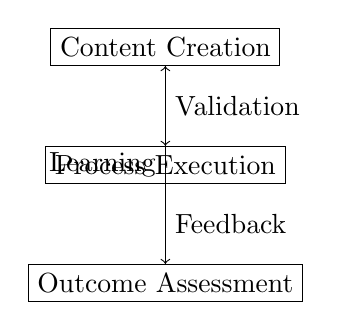
\begin{tikzpicture}[node distance=1.5cm, auto]
    \node (A) [draw, align=center] {Content Creation};
    \node (B) [draw, below of=A, align=center] {Process Execution};
    \node (C) [draw, below of=B, align=center] {Outcome Assessment};

    \path[->] (A) edge node {Validation} (B);
    \path[->] (B) edge node {Feedback} (C);
    \path[->] (C) edge node {Learning} (A);
\end{tikzpicture}
\subsection{Timeline-Budget Integration}
\begin{itemize}
    \item \textbf{Resource Scheduling:}
    \begin{itemize}
        \item Phase Allocations: [Resource timing]
        \item Cost Controls: [Budget tracking]
        \item Adjustment Protocols: [Change management]
    \end{itemize}
\end{itemize}
\section{Budget Management}
\subsection{Financial Cube Structure}

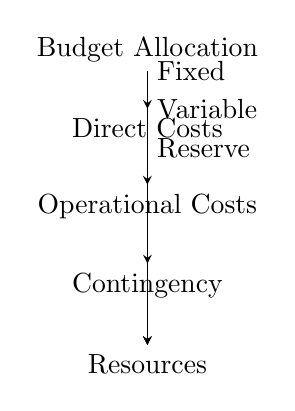
\begin{tikzpicture}[
    node distance = 1cm,
    every node/.style = {align=center},
    >=stealth,
    auto
  ]

  \node (A) {Budget Allocation};
  \node (B) [below of=A] {Direct Costs};
  \node (C) [below of=B] {Operational Costs};
  \node (D) [below of=C] {Contingency};
  \node (E) [below of=D] {Resources};

  \path[->] (A) edge node[above right] {Fixed} (B)
            (A) edge node[above right] {Variable} (C)
            (A) edge node[above right] {Reserve} (D)
            (B) edge (E)
            (C) edge (E)
            (D) edge (E);

\end{tikzpicture}
\subsection{Cost Framework}

\begin{itemize}
    \item Direct Investments:
    \begin{itemize}
        \item Infrastructure Costs:
        \begin{itemize}
            \item Hardware: [Equipment/Devices]
            \item Software: [Licenses/Tools]
            \item Network: [Connectivity/Setup]
        \end{itemize}
        \item Human Resources:
        \begin{itemize}
            \item Core Team: [Roles/Compensation]
            \item External Support: [Consultants/Services]
            \item Training: [Capability Development]
        \end{itemize}
    \end{itemize}
    \item Operational Expenses:
    \begin{itemize}
        \item Running Costs:
        \begin{itemize}
            \item Maintenance: [Regular upkeep]
            \item Utilities: [Service costs]
            \item Consumables: [Regular supplies]
        \end{itemize}
        \item Service Costs:
        \begin{itemize}
            \item Subscriptions: [Regular services]
            \item Support: [Ongoing assistance]
            \item Updates: [Regular improvements]
        \end{itemize}
    \end{itemize}
\end{itemize}
\subsection{Budget Control Mechanisms}
\begin{itemize}
    \item Monitoring System:
    \begin{itemize}
        \item Tracking Methods:
        \begin{itemize}
            \item Cost Centers: [Budget units]
            \item Expense Categories: [Type classification]
            \item Time Periods: [Duration tracking]
        \end{itemize}
        \item Control Points:
        \begin{itemize}
            \item Thresholds: [Limit markers]
            \item Alerts: [Warning systems]
            \item Approvals: [Authorization levels]
        \end{itemize}
    \end{itemize}
    \item Adjustment Protocol:
    \begin{itemize}
        \item Variance Management:
        \begin{itemize}
            \item Detection: [Monitoring points]
            \item Analysis: [Impact assessment]
            \item Response: [Corrective actions]
        \end{itemize}
        \item Reallocation Process:
        \begin{itemize}
            \item Criteria: [Decision factors]
            \item Methods: [Transfer protocols]
            \item Documentation: [Record keeping]
        \end{itemize}
    \end{itemize}
\end{itemize}
\section{Timeline Management}
\subsection{Temporal Cube Structure}
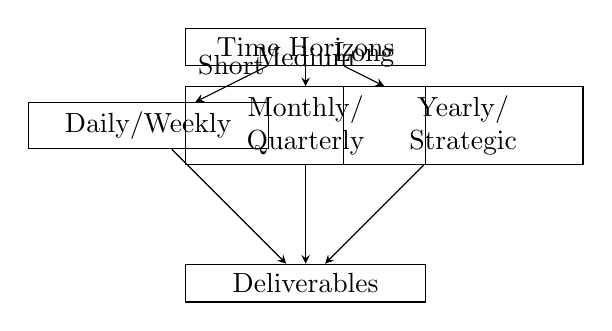
\begin{tikzpicture}[
    node distance = 1cm,
    every node/.style = {align=center},
    block/.style = {rectangle, draw, text width=8em},
    > = stealth,
  ]
    \node[block] (A) {Time Horizons};
    \node[block, below of=A, xshift=-2cm] (B) {Daily/Weekly};
    \node[block, below of=A, xshift=0cm] (C) {Monthly/\\Quarterly};
    \node[block, below of=A, xshift=2cm] (D) {Yearly/\\Strategic};
    \node[block, below of=C,yshift = -1cm] (E) {Deliverables};

    \path[->]
    (A) edge node[above] {Short} (B)
    (A) edge node[above] {Medium} (C)
    (A) edge node[above] {Long} (D)
    (B) edge (E)
    (C) edge (E)
    (D) edge (E);

\end{tikzpicture}
\subsection{Schedule Framework}

\begin{itemize}
    \item Operational Timeline:
    \begin{itemize}
        \item Daily Operations:
        \begin{itemize}
            \item Tasks: [Regular activities]
            \item Checkpoints: [Daily reviews]
            \item Updates: [Status reports]
        \end{itemize}
        \item Weekly Cycles:
        \begin{itemize}
            \item Sprints: [Work packages]
            \item Reviews: [Progress checks]
            \item Planning: [Next steps]
        \end{itemize}
    \end{itemize}

    \item Strategic Timeline:
    \begin{itemize}
        \item Monthly Milestones:
        \begin{itemize}
            \item Objectives: [Key targets]
            \item Reviews: [Achievement checks]
            \item Adjustments: [Course corrections]
        \end{itemize}
        \item Quarterly Goals:
        \begin{itemize}
            \item Targets: [Major objectives]
            \item Assessments: [Performance reviews]
            \item Strategies: [Approach updates]
        \end{itemize}
    \end{itemize}
\end{itemize}
\subsection{Timeline Control System}
\begin{itemize}
    \item Progress Tracking:
    \begin{itemize}
        \item Monitoring Points:
        \begin{itemize}
            \item Daily Standups: [Quick updates]
            \item Weekly Reviews: [Detailed checks]
            \item Monthly Reports: [Comprehensive reviews]
        \end{itemize}
        \item Milestone Tracking:
        \begin{itemize}
            \item Status: [Progress indicators]
            \item Dependencies: [Related items]
            \item Risks: [Potential issues]
        \end{itemize}
    \end{itemize}
    \item Adjustment Mechanisms:
    \begin{itemize}
        \item Schedule Management:
        \begin{itemize}
            \item Variance Analysis: [Delay assessment]
            \item Impact Studies: [Effect evaluation]
            \item Recovery Plans: [Correction strategies]
        \end{itemize}
        \item Resource Alignment:
        \begin{itemize}
            \item Capacity Planning: [Resource matching]
            \item Workload Balancing: [Effort distribution]
            \item Priority Updates: [Focus adjustment]
        \end{itemize}
    \end{itemize}
\end{itemize}
\subsection{Integration Points}
\begin{itemize}
    \item Budget-Timeline Correlation:
    \begin{itemize}
        \item Cost-Schedule Matrix:
        \begin{itemize}
            \item Resource Timing: [Allocation schedule]
            \item Cost Flows: [Expense timing]
            \item Value Delivery: [Benefit realization]
        \end{itemize}
        \item Control Integration:
        \begin{itemize}
            \item Joint Reviews: [Combined assessments]
            \item Unified Reporting: [Integrated updates]
            \item Coordinated Actions: [Synchronized responses]
        \end{itemize}
    \end{itemize}
\end{itemize}
\section{Conclusion}
\subsection{Summary of Achievements}
\begin{itemize}
    \item \textbf{Key Accomplishments:}
    \begin{itemize}
        \item Objectives Met: [Completed goals]
        \item Value Delivered: [Benefits realized]
        \item Innovations: [New approaches]
    \end{itemize}
\end{itemize}
\subsection{Lessons Learned}
\begin{itemize}
    \item \textbf{Success Factors:}
    \begin{itemize}
        \item Effective Practices: [What worked well]
        \item Team Dynamics: [Collaboration insights]
        \item Tools \& Methods: [Useful approaches]
    \end{itemize}

    \item \textbf{Areas for Improvement:}
    \begin{itemize}
        \item Challenges: [Obstacles encountered]
        \item Solutions: [How issues were resolved]
        \item Recommendations: [Future improvements]
    \end{itemize}
\end{itemize}
\subsection{Future Directions}
\begin{itemize}
    \item \textbf{Next Steps:}
    \begin{itemize}
        \item Immediate Actions: [Short-term tasks]
        \item Strategic Plans: [Long-term goals]
        \item Resource Needs: [Required support]
    \end{itemize}
    \item \textbf{Growth Opportunities:}
    \begin{itemize}
        \item Scaling Potential: [Expansion possibilities]
        \item Innovation Areas: [New directions]
        \item Partnership Options: [Collaboration prospects]
    \end{itemize}
\end{itemize}
\section{Appendix}
\subsection{References}
\begin{itemize}
    \item \textbf{Documentation:}
    \begin{itemize}
        \item Technical Specs: [Links]
        \item Process Guides: [Links]
        \item Evidence Records: [Links]
    \end{itemize}
\end{itemize}
\subsection{Change Log}
\begin{itemize}
    \item \textbf{Version History:}
    \begin{itemize}
        \item Changes: [Modifications]
        \item Rationale: [Reasons]
        \item Approvals: [Authorizations]
    \end{itemize}
\end{itemize}
\end{document}